%%%%%%%%%%%%%%%%%%%%%%%%%%%%%%%%%%%%%%%%%%%%%%%%%%%%%%%%%%%%%%%%%%%%%%%%%%%%%%%%
%%%%%%%%%%%%%%%%%%%%%%%%%%%%%%%%%%%%%%%%%%%%%%%%%%%%%%%%%%%%%%%%%%%%%%%%%%%%%%%%
%%% Template for AIMS Rwanda Assignments         %%%              %%%
%%% Author:   AIMS Rwanda tutors                             %%%   ###        %%%
%%% Email: tutors2018-19@aims.ac.rw                               %%%   ###        %%%
%%% Copyright: This template was designed to be used for    %%% #######      %%%
%%% the assignments at AIMS Rwanda during the academic year %%%   ###        %%%
%%% 2018-2019.                                              %%%   #########  %%%
%%% You are free to alter any part of this document for     %%%   ###   ###  %%%
%%% yourself and for distribution.                          %%%   ###   ###  %%%
%%%                                                         %%%              %%%
%%%%%%%%%%%%%%%%%%%%%%%%%%%%%%%%%%%%%%%%%%%%%%%%%%%%%%%%%%%%%%%%%%%%%%%%%%%%%%%%
%%%%%%%%%%%%%%%%%%%%%%%%%%%%%%%%%%%%%%%%%%%%%%%%%%%%%%%%%%%%%%%%%%%%%%%%%%%%%%%%


%%%%%% Ensure that you do not write the questions before each of the solutions because it is not necessary. %%%%%% 

\documentclass[12pt,a4paper]{article}

%%%%%%%%%%%%%%%%%%%%%%%%% packages %%%%%%%%%%%%%%%%%%%%%%%%
\usepackage{amsmath}
\usepackage{amssymb}
\usepackage{amsthm}
\usepackage{amsfonts}
\usepackage{graphicx}
\usepackage[all]{xy}
\usepackage{tikz}
\usepackage{verbatim}
\usepackage[left=2cm,right=2cm,top=3cm,bottom=2.5cm]{geometry}
\usepackage{hyperref}
\usepackage{caption}
\usepackage{subcaption}
\usepackage{psfrag}
\usepackage{multicol}
\usepackage{tabularx}
\usepackage{enumitem}
\usepackage{csvsimple}
\usepackage{booktabs}
\usepackage{colortbl}
\usepackage{tabulary}
\usepackage{etoolbox}

%%%%%%%%%%%%%%%%%%%%% students data %%%%%%%%%%%%%%%%%%%%%%%%
\newcommand{\student}{Kamau Gladys Muthoni}
\newcommand{\course}{Research Methods in Climate Science}
\newcommand{\assignment}{1}

%%%%%%%%%%%%%%%%%%% using theorem style %%%%%%%%%%%%%%%%%%%%
\newtheorem{thm}{Theorem}
\newtheorem{lem}[thm]{Lemma}
\newtheorem{defn}[thm]{Definition}
\newtheorem{exa}[thm]{Example}
\newtheorem{rem}[thm]{Remark}
\newtheorem{coro}[thm]{Corollary}
\newtheorem{quest}{Question}[section]

%%%%%%%%%%%%%%  Shortcut for usual set of numbers  %%%%%%%%%%%

\newcommand{\N}{\mathbb{N}}
\newcommand{\Z}{\mathbb{Z}}
\newcommand{\Q}{\mathbb{Q}}
\newcommand{\R}{\mathbb{R}}
\newcommand{\C}{\mathbb{C}}

%%%%%%%%%%%%%%%%%%%%%%%%%%%%%%%%%%%%%%%%%%%%%%%%%%%%%%%555
\begin{document}

%%%%%%%%%%%%%%%%%%%%%%% title page %%%%%%%%%%%%%%%%%%%%%%%%%%
\thispagestyle{empty}
\begin{center}
\textbf{AFRICAN INSTITUTE FOR MATHEMATICAL SCIENCES \\[0.5cm]
(AIMS RWANDA, KIGALI)}
\vspace{1.0cm}
\end{center}

%%%%%%%%%%%%%%%%%%%%% assignment information %%%%%%%%%%%%%%%%
\noindent
\rule{17cm}{0.2cm}\\[0.3cm]
Name: \student \hfill Assignment Number: \assignment\\[0.1cm]
Course: \course \hfill Date: \today\\
\rule{17cm}{0.05cm}
\vspace{1.0cm}

\section{Task 1: Cluster Analysis}
\section{Introduction}
The data choosen for this study was extracted from Climate Dataset (CRU) over Turkana City in Kenya with coordinates 3.3122$^\text{o}$ N, 35.5658$^\text{o}$ E. 
The study is based on the month of April which was recorded with the highest amount of precipitation over the span of 51 years from 1960 to 2010. The aim of the study is to identify the characteristics of three Cluster Analysis algorithms. CA groups climate variables into groups of similar type. The importance of this study is to learn how different methods of hierarchical cluster analysis work. 

\begin{figure}[h]
	\centering
	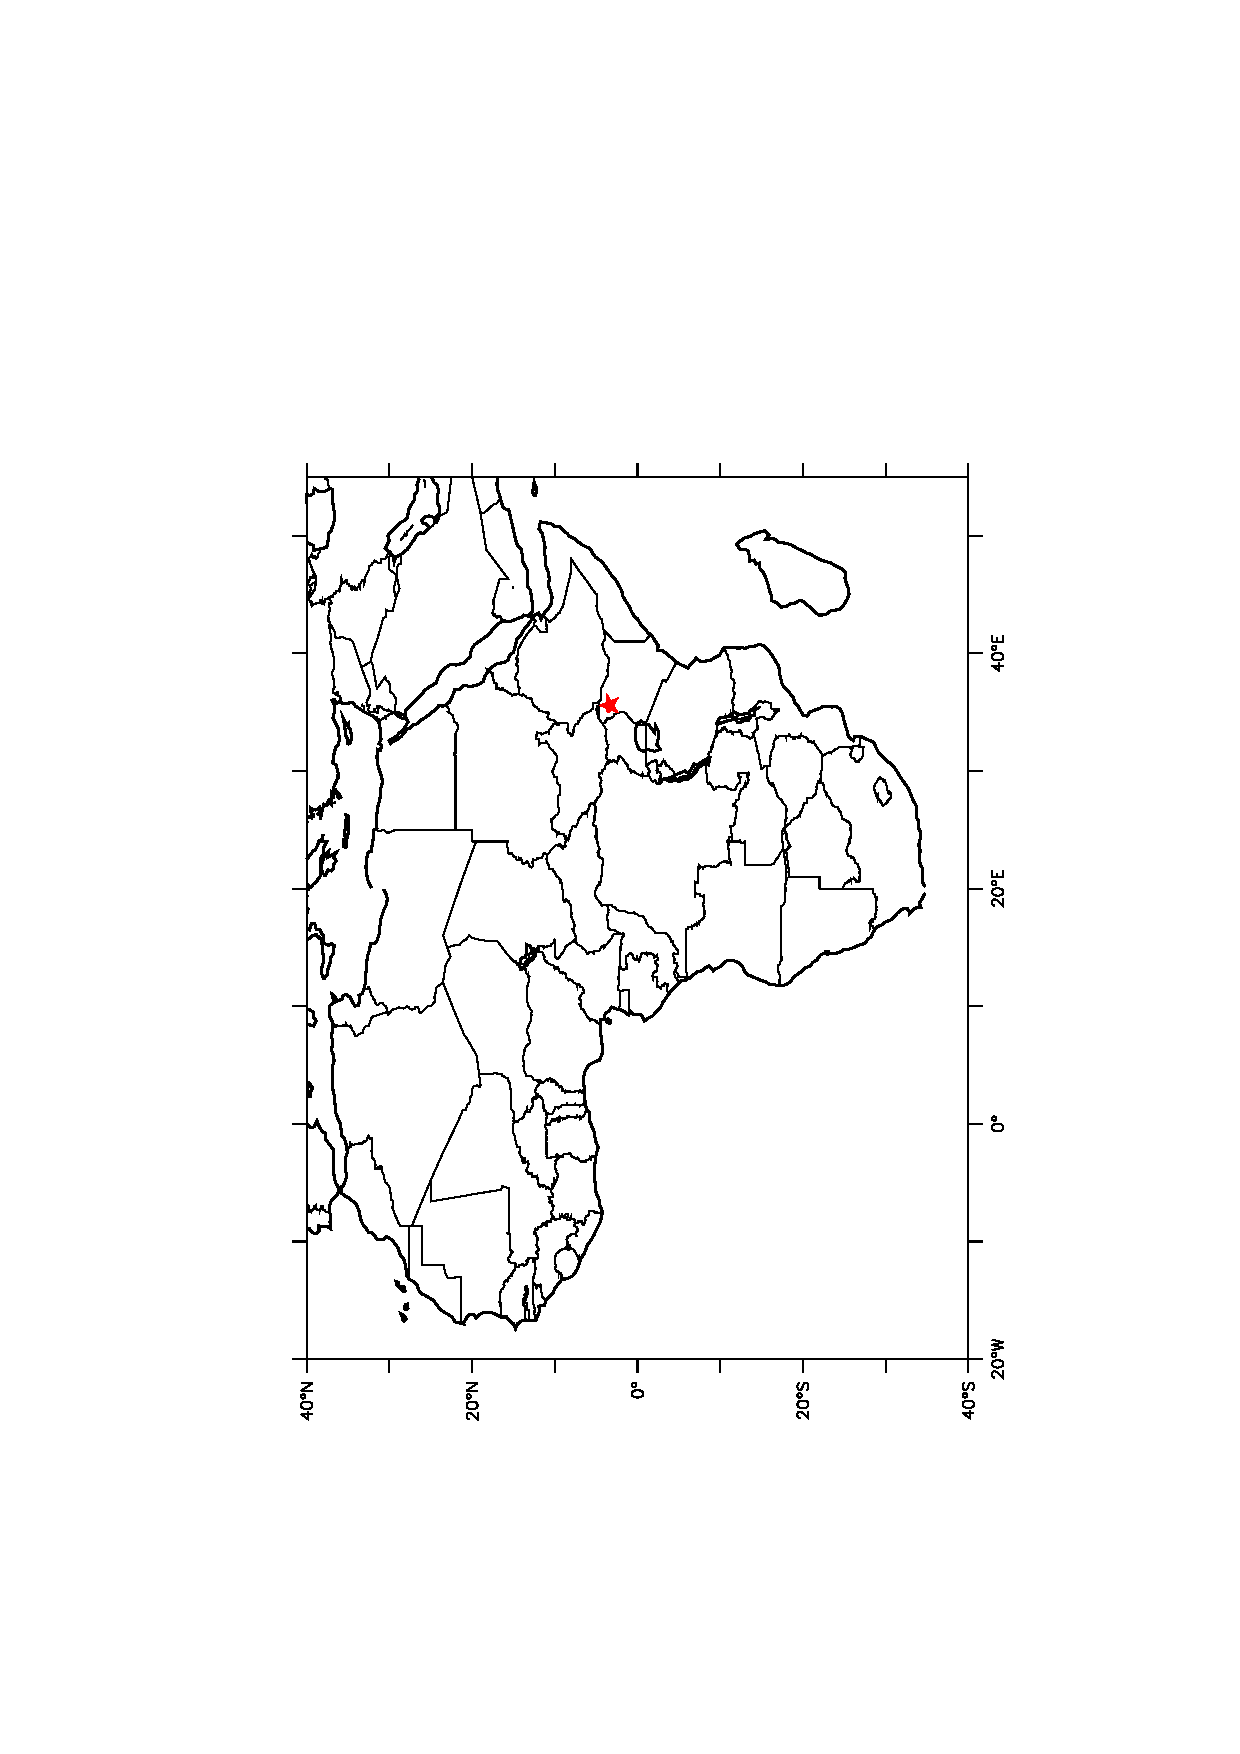
\includegraphics[width=0.8\linewidth]{Turkana}
	\caption{}
	\label{fig:turkana}
\end{figure}
\noindent There's no clear history of analysing climate data of Turkana using CA. This study therefore groups the various climate variables over Turkana city.\\

\noindent The extracted data had 51 rows and 10 columns with the following key variables:
\begin{itemize}
	\item CLDD - Cloud Cover Days
	\item PRED - Precipitation Days
	\item WETD - Wet Days
	\item  VAPD - Vapour Pressure
	\item TMND - Minimum Temperature
	\item TMPD - Mean Temperature
	\item TMXD - Maximum Temperature
	\item PETD - Potential Evapotranspiration
	\item DTRD - Diurnal Temperature Range
\end{itemize}

 
\section{Methodology} 
 After extracting the needed data using microsoft excel it was subjected to CA analysis methods. This study focused on 3 hierarchical CA methods; single linkage, average linkage and ward algorithm. Vertical cluster tress was the main tool used to visualise the data. R was used as the programming software and language to up with the cluster trees. Clustering was done by grouping the data matrix to explore the grouping of climate variable and years (1960 -2010) over the city.
\section{Results and Interpretation}
The data was analysed using Hierarchical cluster method which comprises of single linkage, average linkage and ward algorithm. The study explores the grouping of climate variables and years.


\subsection{Climate Viariables}
\begin{enumerate}[label=\roman*)]
	\item Single Linkage

\noindent Starts with two closest data points and link. Next two closest data points and link until all data points were linked as shown in figure \ref{fig:rplots1}.


\begin{figure}[h]
	\centering
	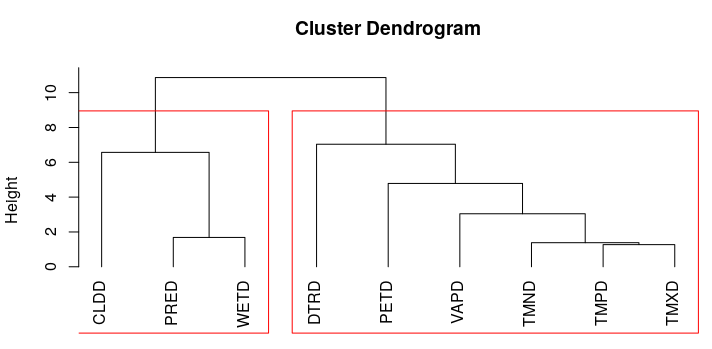
\includegraphics[width=0.7\linewidth]{S1}
	\caption{Single linkage}
	\label{fig:rplots1}
\end{figure}
\noindent Cutting the cluster tree at height 9 creates two groups:
\begin{itemize}
	\item CLDD, PRED, WETD - common feature is wetness.
	\item DTRD, PETD, VAPD, TMND, TMPD, TMXD - common feature is temparature.
\end{itemize} 
PRED and WETD are more similar to each other compared to CLDD indicated by the short linkage distance. TMPD, TMXD and TMPD are also more similar to each other than VAPD, PETD and DTRD.

\item Average Linkage

\noindent Similar to single linkage but based on the average linkage distance. Grouped the data as shown in figure \ref{fig:a1}.

\begin{figure}[h]
	\centering
	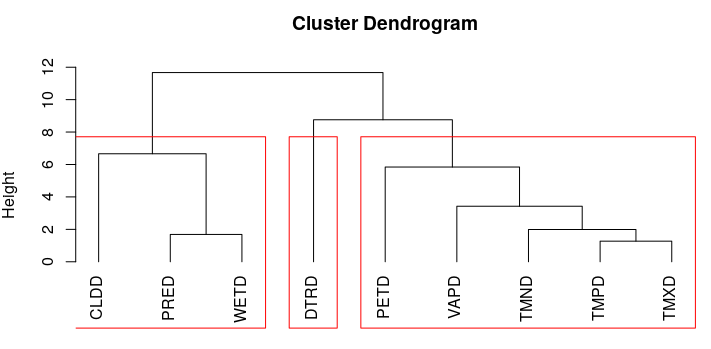
\includegraphics[width=0.7\linewidth]{A1}
	\caption{Average linkage}
	\label{fig:a1}
\end{figure}
\noindent Cutting the cluster tree at the height of almost 8 created 3 groups:
\begin{itemize}
	\item CLDD, PRED, WETD - common feature is wetness.
	\item DTRD
	\item PETD, VAPD, TMND, TMPD, TMXD - common featrue is temperature.
\end{itemize}
DTRD is an outlier. PRED and WETD are more similar to each other compared to CLDD which joins the cluster later. TMPD and TMXD are also more similar to each other more compared to PETD, VAPD and TMND.

\item Ward Algorithm

\noindent Based on variance analysis. It seeks to minimize within group variance and maximize between group variance. Grouped the data as shown in figure \ref{fig:w1}.

\begin{figure}[h]
	\centering
	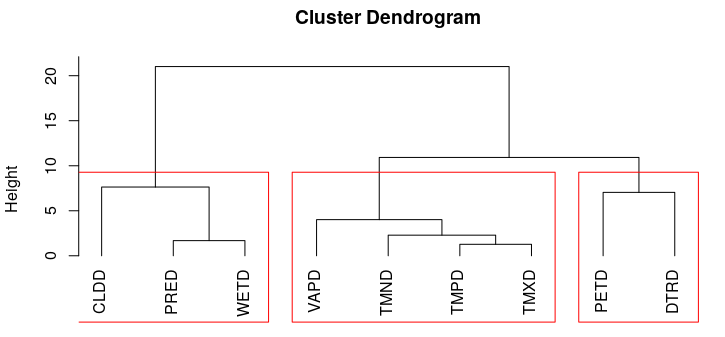
\includegraphics[width=0.7\linewidth]{W1}
	\caption{Ward algorithm}
	\label{fig:w1}
\end{figure}
\noindent Cutting the cluster tree at the height of almost 10 created 3 groups:
\begin{itemize}
	\item CLDD, PRED, WETD -  common feature is wetness.
	\item PETD, DTRD - potential evapotranspiration causes diurnal tempareture change.
	\item  VAPD, TMND, TMPD, TMXD - common feature is temperature.
\end{itemize}
DTRD and PETD are of similar type. PRED and WETD are more similar to each other compared to CLDD which joins the cluster later. TMPD and TMXD are also more similar to each other more compared to VAPD and TMND.
\end{enumerate}

\subsection{Years (1960 -2010)}
\begin{enumerate}[label=\roman*)]

\item Single Linkage

\noindent Grouped the data points of years as shown in figure \ref{fig:s2}.
\begin{figure}[h]
	\centering
	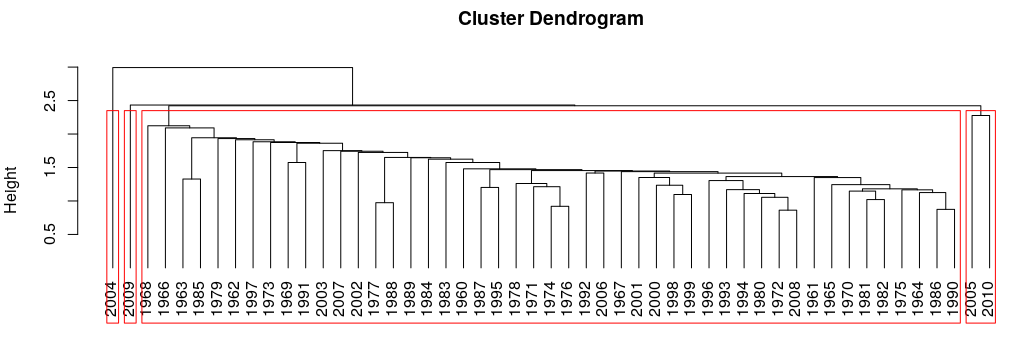
\includegraphics[width=0.7\linewidth]{S2}
	\caption{Single linkage}
	\label{fig:s2}
\end{figure}
Cutting the cluster tree at the height of almost 2.5 groups the data points into 2 clusters with 2004 and 2009 as outliers. The largest group captures most of the data points indicating that all the years in this group share a common feature. It is also evident from the cluster tree that 1977 and 1988, 1974 and 1976, 1972 and 2008, 1986 and 1990 are more similar to each other since they are closest to each other.\\

\item Average Linkage

\noindent Data points of years were grouped as shown in figure \ref{fig:A2}.

Cutting the cluster tree at the height of 3.5 groups the data points into 6 clusters with 2004 as an outliers. The 2 largest group captures most of the data points indicating that all the years in these groups share a common feature respectively.
\begin{figure}[h]
	\centering
	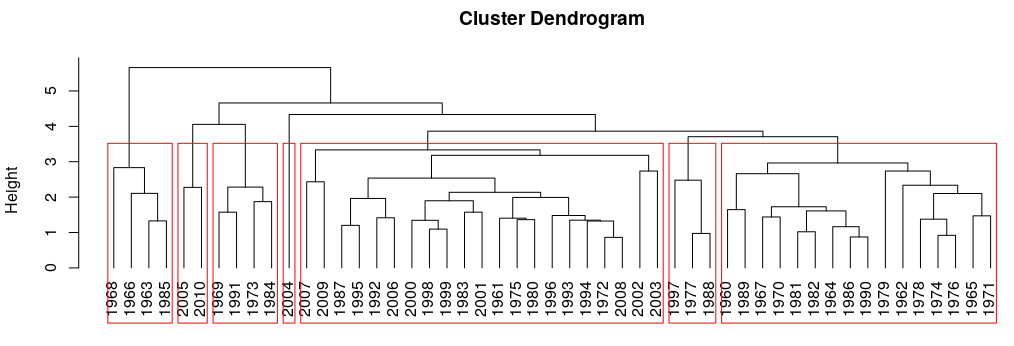
\includegraphics[width=0.7\linewidth]{A2}
	\caption{Average linkage}
	\label{fig:A2}
\end{figure}\\
\item Ward Algorithm

\noindent Grouped the data points of years as shown in figure \ref{fig:w2}.
Cutting the cluster tree at the height of 7 groups the data points into 6 clusters.

\begin{figure}[h]
	\centering
	\includegraphics[width=0.7\linewidth]{w2}
	\caption{Ward algorithm}
	\label{fig:w2}
\end{figure}

\section{Conclusion}
\noindent From the three hierarchical cluster analysis methods used in the 2 cases of variables its clear that single linkage and average linkages identify the outliers but the groups are not well defined. Ward algorithm clearly defines the groups but outliers are not well identified. It is also noted that cluster trees for climate variables and year variables are different.The years grouped together indicate that the climate feature was common to those years.
\end{enumerate}

\section{Task 2: Principal Component Analysis (PCA)}
\section{Introduction}

PCA is a procedure that focuses on dimesionality reduction. It extracts fewer and independent underlying dimensions around which the data variance is organised. It also identifies the main processes that explain the largest percentage variance of the dataset. The aim of the task is to study the characteristics of PCA and compare them with that of CA. The main importance of this tast is to learn how PCA works.  PCA has been used on various studies like climate variability and change on vulnerability and adaptation among Turkana pastoralists, establishing vegetable cover change over time and assessing the impact of climate change on food security of communities in Turkana. This study will try to get a deeper insight of Turkana climate data and explain the main processes that the city has been experiencing over a span of 51years.

\section{Methodology}
The study used two methods of dimentionality reduction; rotated and non-rotated. These two methods had different outputs but rotated was more efficient in reducing the number of dimensions. It allows changing of the factor analysis to identify new patterns of the factor structure while unrotated PCA tries to illustrate the maximum variance value with minimal number of factors. Rotated PCA helps to extract meaningful adat that accurately represents the original dataset. The study looked at component loadings, variation and component scores to select the most important principal factors and better understand the dataset. The results were compared to ward algorithm to better understand PCA. R software was used for programming.

\section{Results and Interpretation}

\begin{enumerate}[label=\roman*)]
	\item Variation (Rotated and Unrotated PCA)\\
	 A total of 9 principle components were obtained as shown in table \ref{ps1}. The standard deviation measures variability across each principle component. Proportion of variance is the total variance percentage explained by each principle component in the original data set. PC1 explains 50\% of the total variance in the original dataset. PC2 explains 23\% of the total variance. In cumulative proportion PC1,PC2 and PC4 explains 85\% of the total variance. As a result PC1, PC2 and PC4 were selected to explain the dataset thus dimentionality reduction.\\
Both unrotated and rotated differ in principle components that best describe the data set. Rotated method was prefered to unrotated as it reduces the dimensions to PC1,PC2 and PC4 which explain a variance of 44\%, 23\% and 18\% respectively.
\newpage
\begin{table}[h]
	\centering
	\begin{tabular}{|l|l|l|l|l|l|l|}
	\hline
	& \multicolumn{3}{l|}{\textbf{Unrotated}}                                                                                                                                   & \multicolumn{3}{l|}{\textbf{Rotated}}                                                                                                                                     \\ \cline{2-7} 
& \textbf{Std dev} & \textbf{\begin{tabular}[c]{@{}l@{}}Proportion\\  of Variance\end{tabular}} & \textbf{\begin{tabular}[c]{@{}l@{}}Cumulative\\  Proportion\end{tabular}} & \textbf{Std dev} & \textbf{\begin{tabular}[c]{@{}l@{}}Proportion \\ of Variance\end{tabular}} & \textbf{\begin{tabular}[c]{@{}l@{}}Cumulative \\ Proportion\end{tabular}} \\ \hline
	\textbf{PC1}       & 2.276            & 0.576                                                                      & 0.576                                                                     & 3.947            & {\color[HTML]{FE0000} 0.453}                                               & 0.453                                                                     \\ \hline
	\textbf{PC2}       & 1.419            & 0.224                                                                      & 0.800                                                                     & 2.082            & {\color[HTML]{FE0000} 0.261}                                               & 0.714                                                                    \\ \hline
	\textbf{PC3}       & 1.048            & 0.122                                                                      & 0.922                                                                     & 1.622            & {\color[HTML]{FE0000} 0.213}                                               & {\color[HTML]{FE0000} 0.927}                                              \\ \hline
	\textbf{PC4}       & 0.722            & 0.058                                                                      & 0.979                                                                     & 1.152            &  0.053                                              &  0.980                                             \\ \hline
	\textbf{PC5}       & 0.386            & 0.017                                                                      & 0.996                                                                     & 0.156            & 0.012                                                                      & 0.992                                                                    \\ \hline
	\textbf{PC6}       & 0.163            & 0.005                                                                      & 0.997                                                                    & 0.027            & 0.005                                                                     & 0.997                                                                     \\ \hline
	\textbf{PC7}       & 0.093            & 0.001                                                                      & 1                                                                         & 0.014            & 0.003                                                                      & 1.000                                                                     \\ \hline
	\textbf{PC8}       & 0.025            & 0                                                                          & 1                                                                         & 0.001            & 0                                                                          & 1.000                                                                     \\ \hline
	\textbf{PC8}       & 0.025            & 0                                                                          & 1                                                                         & 0.001            & 0                                                                          & 1.000                                                                     \\ \hline
	\textbf{PC9}       & 2.635            & 0                                                                          & 1                                                                         & 0                & 0                                                                          & 1.00                                                                      \\ \hline
	\end{tabular}
\caption{PCA Summary}
\label{ps1}
\end{table}

\noindent Selection of the most important principle components can also be selected using the scree plot show in \ref{fig:screep} with a default setting that the varinace should be atleast 1.


\begin{figure}[h]
	\centering
	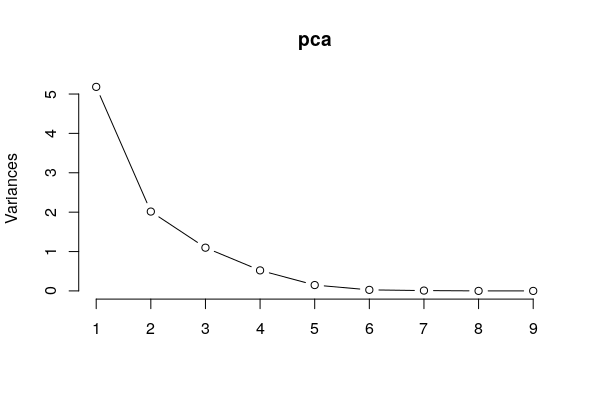
\includegraphics[width=0.7\linewidth]{ScreeP}
	\caption{}
	\label{fig:screep}
\end{figure}

\item Component Loadings (Rotated)\\
These are the correlation coefficients of the linear combination of the original variables from which principle components are constructed.
Rotated PCA determines the loadings cutoff for the importnat variables that contribute highest to the factors as shown in red in table \ref{load}.
\begin{table}[h]
	\centering
	\begin{tabular}{|l|l|l|l|}
		\hline
		\textbf{Variables} & \textbf{PC1}                    & \textbf{PC2}                     & \textbf{PC3}                     \\ \hline
		\textbf{PRED}      & -0.162010                       & {\color[HTML]{FE0000} -0.953727} & -0.171107                        \\ \hline
		\textbf{PETD}      & 0.546160                        & 0.396223                         & 0.678831                         \\ \hline
		\textbf{CLDD}      & -0.141978                       & -0.508158                        & {\color[HTML]{FE0000} -0.714389} \\ \hline
		\textbf{DTRD}      & 0.011618                        & 0.029256                         & {\color[HTML]{FE0000} 0.893948}  \\ \hline
		\textbf{TMPD}      & {\color[HTML]{FE0000} 0.965685} & 0.142101                         & 0.194406                         \\ \hline
		\textbf{TMND}      & {\color[HTML]{FE0000} 0.983804} & 0.137589                         & 0.028010                         \\ \hline
		\textbf{TMXD}      & {\color[HTML]{FE0000} 0.917354} & 0.138291                         & 0.349367                         \\ \hline
		\textbf{VAPD}      & {\color[HTML]{FE0000} 0.935681} & 0.154074                         & -0.057063                        \\ \hline
		\textbf{WETD}      & -0.167719                       & {\color[HTML]{FE0000} -0.952899} & -0.155570                        \\ \hline
	\end{tabular}
\caption{Principle component loadings}
\label{load}
\end{table}

TMPD, TMND, TMXD and VAPD all increase in PC1. Due to the high temperatures in the dataset, this process is drought.  In PC2 both PRED and WETD decreases. In drought seaons there's no rain and the land is dry. In PC3 as CLDD decreases,DTRD increases. When there's no cloud during the night the temparatures tend to decrease and increase during the day. This results to increase in dirunal range temparatures.
\newpage
\item Component Scores (Rotated)\\
Figure \ref*{fig:scores} figuratively describes percentage variance of each principle component on the original data and the component scores. The score shows how each process varies in different years. PC1 most active in 2010, most inactive in 1968 but was dormant in 1975. PC2 was most active in 1966, most inactive in 1969 but was dormant in 1960,1961 and 2002. PC4 most active in 2005, most inactive in 1963 with no dormance in any year.

\newpage

\begin{figure}[h]
	%\centering
	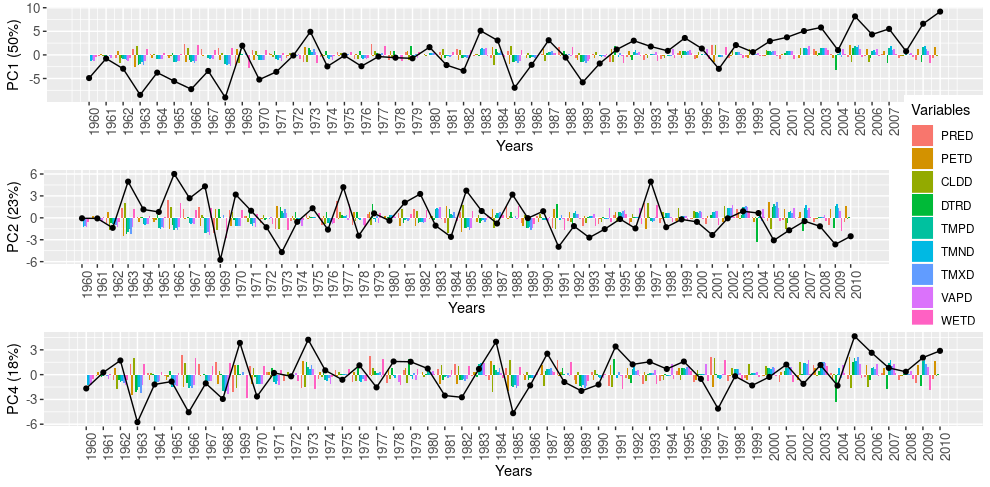
\includegraphics[width=1.1\linewidth, height=0.5\textheight]{scores}
	\caption{Component scores}
	\label{fig:scores}
\end{figure}

\end{enumerate}


\section{Conclusion}

PCA analysis identifies the processes that cause the climate variables to vary. PCA gives a deeper understanding of the dataset as it aslo reduces dimentionality which can be helpful for better climate predictions and data analysis. 
Both loadings and scores play an important role in analysing data using PCA. Ward algorithm defines the groups well but you can barely deduce how they are grouped and the processes involved.

\newpage
\section{Task 3: Time-Series Analysis }
\section{Introducttion}
Time series analysis is a sequence of data(continuous) that follow non-random orders. The data must be equally spaced time intervals. To deploy time series analysis the dataset must satisfy these two conditions. Time series analysis comprises of various methods that analysizes time series data for the purpose of extracting meaningful climate statistics and other featurs of the data. The aim of this task was to explore the time series patterns in precipitation (PRED) and temperature (TMPD) data and the relationships between the two variables. This is important for the purpose of learning and analysing the patterns of temperature and precicpitation in Turkana city over a span of 51years from 1960-2010. As a result it helps to study the past and predict the future.

\section{Methodology}
There are various methods of time series analysis which can be classified into frequency domain (Fourier and Wavelet analysis ) and time domain (autocorrelation and cross-correlation). This task focused on time domain and time series to identify if there was trend in the data. Dataset was re-extracted again using excel so as to include the month variable since the data was indexed monthly from January 1960 to December 2010. Using statistica TMPD and PRED values were subjected to time series to identify the patterns. At some point it was required to detrend the temperature variable for better analysis of the data. Detrending of the data was done using microsoft Excel.
\section{Results and Interpretation}

\subsection{Plot of PRED and TMPD time series}
It was evident from figure \ref{fig:trended-tmpd} that temperature variable had deterministic and global trend; change in mean over time. Line of best fit showed the temperature values were increasing with 0.0025$^0$C every month from 1960 to 2010. Precipitation variable presented a very small trend as shown in figure \ref{fig:timeseries-pred} which was neglected. This implied the slope of the best line of fit was insignificant but we can see the pattern of highest amount of rainfall recorded at 120 was recieved in 1960 and this has reduced over the years.
\newpage
\begin{figure}[h]
	\centering
	\includegraphics[width=0.7\linewidth, height=0.3\textheight]{"../Assignment 2/Trended TMPD"}
	\caption{}
	\label{fig:trended-tmpd}
\end{figure}

\begin{figure}[h]
	\centering
	\includegraphics[width=0.7\linewidth, height=0.3\textheight ]{"../Assignment 2/TimeSeries PRED"}
	\caption{}
	\label{fig:timeseries-pred}
\end{figure}
\newpage
\subsection{Detrended TMPD}
\begin{figure}[h]
	\centering
	\includegraphics[width=0.7\linewidth]{"../Assignment 2/Detrended TMPD"}
	\caption{Detrended TMPD}
	\label{fig:detrended-tmpd}
\end{figure}
\noindent There are many methods of detrending data but linear regression was used in this case. Detrending was done to remove distortion in TMPD variable to allow better analysis of its variability. Plot of the detrended data gave a clearer visual of the cyclic patterns that is increase and decrease of temperature with time compared to trended data. It was clear to identify extreme maximum temperature of ......

\subsection{Correlogram for PRED and DTMPD}
Correlogram is synonym for autocorrelation. It is the correlation between a series data and lagged version of itself. It is used to find repeating patterns. As shown in figure \ref{fig:autocorrelation-dtmpd} DTMPD autocorrelation shows a significant sinusidal cycle. With a lag of 1 month, it shows that temperature data is correlated with the past data and it varies with time. It also shows a repetitive annual pattern. The red line indicates the approximate 95\% confidence interval.\\

\noindent Figure \ref{fig:autocorrelation-pred} shows a weak sinosidal autocorrelation of precipitation. At lag 1 correlation is at approximately 0.25. This shows that the correlation is less significant and precipitation values are almost random in the area.
\begin{figure}[h]
	\centering
	\includegraphics[width=0.7\linewidth, height=0.2\textheight]{"../Assignment 2/Autocorrelation DTMPD"}
	\caption{Autocorrelation DTMPD}
	\label{fig:autocorrelation-dtmpd}
\end{figure}

\begin{figure}[h]
	\centering
	\includegraphics[width=0.7\linewidth, height=0.3\textheight]{"../Assignment 2/Autocorrelation PRED"}
	\caption{Autocorrelation PRED}
	\label{fig:autocorrelation-pred}
\end{figure}

\newpage

\subsection{Cross-correlation of PRED and DTMPD}
Cross-correlation describes the degree of correlation between two different time series. It is useful in determining whether changes in one time series has effect on the other time series. Figure \ref{fig:crosscorrelation} shows temperature is signficantly correlated to precicpitation. At lag -13 and 11 the correlation is 0.5. This implies that increase in temperature increases the level of evaporation which can later condense to form clouds which can lead rainfall.
\begin{figure}[h]
	\centering
	\includegraphics[width=0.7\linewidth]{"../Assignment 2/CrossCorrelation "}
	\caption{}
	\label{fig:crosscorrelation}
\end{figure}

\newpage
\section{Conclusion}
Autocorrelation, cross-correlation and time series played a vital role in identifying the underlying patterns of how temperature and precipitation varied with time. To get a deeper and better insight of the data more analysis needs to be done. Both autocorrelation an dcross-correlation are based on correlation.















\section{Task 4: Spectral and Wavelet Analysis}
\section{Introduction}
Spectral analysis is also referred to as fourier analysis. It is useful in identifying seasonal fluctuatins of different lengths in the dataset. From the cyclic pattern identified in fourier analysis, wavelet analysis explains the behaviour and change of the cycles and amplitude with time. The aim of this task is to explore and compare spectral analysis and wavelet analysis using the precipitation data. The study was important for learning and analysing how the cycles of precicpation varied within the span of 51years from  1960-2010 in Turakana City. This task will also be an extension of the analysis done in task 3.
\section{Methodology}


\section{Results and Interpretation}
\section{Conclusion}

\end{document}